\documentclass[twoside]{book}

% Packages required by doxygen
\usepackage{fixltx2e}
\usepackage{calc}
\usepackage{doxygen}
\usepackage[export]{adjustbox} % also loads graphicx
\usepackage{graphicx}
\usepackage[utf8]{inputenc}
\usepackage{makeidx}
\usepackage{multicol}
\usepackage{multirow}
\PassOptionsToPackage{warn}{textcomp}
\usepackage{textcomp}
\usepackage[nointegrals]{wasysym}
\usepackage[table]{xcolor}

% Font selection
\usepackage[T1]{fontenc}
\usepackage[scaled=.90]{helvet}
\usepackage{courier}
\usepackage{amssymb}
\usepackage{sectsty}
\renewcommand{\familydefault}{\sfdefault}
\allsectionsfont{%
  \fontseries{bc}\selectfont%
  \color{darkgray}%
}
\renewcommand{\DoxyLabelFont}{%
  \fontseries{bc}\selectfont%
  \color{darkgray}%
}
\newcommand{\+}{\discretionary{\mbox{\scriptsize$\hookleftarrow$}}{}{}}

% Page & text layout
\usepackage{geometry}
\geometry{%
  a4paper,%
  top=2.5cm,%
  bottom=2.5cm,%
  left=2.5cm,%
  right=2.5cm%
}
\tolerance=750
\hfuzz=15pt
\hbadness=750
\setlength{\emergencystretch}{15pt}
\setlength{\parindent}{0cm}
\setlength{\parskip}{0.2cm}
\makeatletter
\renewcommand{\paragraph}{%
  \@startsection{paragraph}{4}{0ex}{-1.0ex}{1.0ex}{%
    \normalfont\normalsize\bfseries\SS@parafont%
  }%
}
\renewcommand{\subparagraph}{%
  \@startsection{subparagraph}{5}{0ex}{-1.0ex}{1.0ex}{%
    \normalfont\normalsize\bfseries\SS@subparafont%
  }%
}
\makeatother

% Headers & footers
\usepackage{fancyhdr}
\pagestyle{fancyplain}
\fancyhead[LE]{\fancyplain{}{\bfseries\thepage}}
\fancyhead[CE]{\fancyplain{}{}}
\fancyhead[RE]{\fancyplain{}{\bfseries\leftmark}}
\fancyhead[LO]{\fancyplain{}{\bfseries\rightmark}}
\fancyhead[CO]{\fancyplain{}{}}
\fancyhead[RO]{\fancyplain{}{\bfseries\thepage}}
\fancyfoot[LE]{\fancyplain{}{}}
\fancyfoot[CE]{\fancyplain{}{}}
\fancyfoot[RE]{\fancyplain{}{\bfseries\scriptsize Generated on Fri Dec 4 2015 14\+:33\+:33 for Elements by Doxygen }}
\fancyfoot[LO]{\fancyplain{}{\bfseries\scriptsize Generated on Fri Dec 4 2015 14\+:33\+:33 for Elements by Doxygen }}
\fancyfoot[CO]{\fancyplain{}{}}
\fancyfoot[RO]{\fancyplain{}{}}
\renewcommand{\footrulewidth}{0.4pt}
\renewcommand{\chaptermark}[1]{%
  \markboth{#1}{}%
}
\renewcommand{\sectionmark}[1]{%
  \markright{\thesection\ #1}%
}

% Indices & bibliography
\usepackage{natbib}
\usepackage[titles]{tocloft}
\setcounter{tocdepth}{3}
\setcounter{secnumdepth}{5}
\makeindex

% Custom commands
\newcommand{\clearemptydoublepage}{%
  \newpage{\pagestyle{empty}\cleardoublepage}%
}


%===== C O N T E N T S =====

\begin{document}

% Titlepage & ToC
\pagenumbering{roman}
\begin{titlepage}
\vspace*{7cm}
\begin{center}%
{\Large Elements \\[1ex]\large 1.\+0.\+1 }\\
\vspace*{1cm}
{\large Generated by Doxygen 1.8.10}\\
\vspace*{0.5cm}
{\small Fri Dec 4 2015 14:33:33}\\
\end{center}
\end{titlepage}
\clearemptydoublepage
\tableofcontents
\clearemptydoublepage
\pagenumbering{arabic}

%--- Begin generated contents ---
\chapter{Hierarchical Index}
\section{Class Hierarchy}
This inheritance list is sorted roughly, but not completely, alphabetically\+:\begin{DoxyCompactList}
\item \contentsline{section}{Del\+Sequence}{\pageref{class_del_sequence}}{}
\item Q\+Main\+Window\begin{DoxyCompactList}
\item \contentsline{section}{Main\+Window}{\pageref{class_main_window}}{}
\end{DoxyCompactList}
\item Q\+Widget\begin{DoxyCompactList}
\item \contentsline{section}{Game}{\pageref{class_game}}{}
\end{DoxyCompactList}
\end{DoxyCompactList}

\chapter{Class Index}
\section{Class List}
Here are the classes, structs, unions and interfaces with brief descriptions\+:\begin{DoxyCompactList}
\item\contentsline{section}{{\bf Del\+Sequence} \\*Delete sequence class, class that stores list of tiles to be deleted }{\pageref{class_del_sequence}}{}
\item\contentsline{section}{{\bf Game} \\*Main class of game, using mainly Q\+Painter to do all painting }{\pageref{class_game}}{}
\item\contentsline{section}{{\bf Main\+Window} }{\pageref{class_main_window}}{}
\end{DoxyCompactList}

\chapter{Class Documentation}
\section{Del\+Sequence Class Reference}
\label{class_del_sequence}\index{Del\+Sequence@{Del\+Sequence}}


The \doxyref{Del\+Sequence}{p.}{class_del_sequence} class the delete sequence class, class that stores list of tiles to be deleted.  




{\ttfamily \#include $<$game.\+h$>$}

\subsection*{Public Member Functions}
\begin{DoxyCompactItemize}
\item 
void {\bf add} (int x, int y)
\begin{DoxyCompactList}\small\item\em \doxyref{Del\+Sequence\+::add}{p.}{class_del_sequence_ad9e5c357e9575ee3cf8cedf9a236dff1} add x and y position to sequence. \end{DoxyCompactList}\item 
std\+::pair$<$ int, int $>$ {\bf operator[$\,$]} (int a)
\begin{DoxyCompactList}\small\item\em \doxyref{Del\+Sequence\+::operator [$\,$]}{p.}{class_del_sequence_a8b0e2cbd0d75c814574bf744e62d8838} directly access elements. \end{DoxyCompactList}\item 
bool {\bf operator==} ({\bf Del\+Sequence} d2)
\begin{DoxyCompactList}\small\item\em \doxyref{Del\+Sequence\+::operator ==}{p.}{class_del_sequence_aaf59c8f7f00ce81886c89e8e414b767b} whether two sequence is same. \end{DoxyCompactList}\end{DoxyCompactItemize}
\subsection*{Public Attributes}
\begin{DoxyCompactItemize}
\item 
Q\+Time {\bfseries t}\label{class_del_sequence_ad80f295c651f81b3288b58cd58157fd7}

\item 
bool {\bfseries score\+\_\+added}\label{class_del_sequence_aba8848520a045e7e6e21dbaae96b9b9a}

\item 
int {\bfseries score\+\_\+inc}\label{class_del_sequence_a0f89aabc76a31a66531f99ea6c038ef8}

\item 
std\+::vector$<$ std\+::pair$<$ int, int $>$ $>$ {\bfseries seq}\label{class_del_sequence_a4988a6eeafdbdd06dd150281e95e9bb8}

\end{DoxyCompactItemize}


\subsection{Detailed Description}
The \doxyref{Del\+Sequence}{p.}{class_del_sequence} class the delete sequence class, class that stores list of tiles to be deleted. 

\subsection{Member Function Documentation}
\index{Del\+Sequence@{Del\+Sequence}!add@{add}}
\index{add@{add}!Del\+Sequence@{Del\+Sequence}}
\subsubsection[{add(int x, int y)}]{\setlength{\rightskip}{0pt plus 5cm}void Del\+Sequence\+::add (
\begin{DoxyParamCaption}
\item[{int}]{x, }
\item[{int}]{y}
\end{DoxyParamCaption}
)\hspace{0.3cm}{\ttfamily [inline]}}\label{class_del_sequence_ad9e5c357e9575ee3cf8cedf9a236dff1}


\doxyref{Del\+Sequence\+::add}{p.}{class_del_sequence_ad9e5c357e9575ee3cf8cedf9a236dff1} add x and y position to sequence. 


\begin{DoxyParams}{Parameters}
{\em x} & x position \\
\hline
{\em y} & y position \\
\hline
\end{DoxyParams}
\index{Del\+Sequence@{Del\+Sequence}!operator==@{operator==}}
\index{operator==@{operator==}!Del\+Sequence@{Del\+Sequence}}
\subsubsection[{operator==(\+Del\+Sequence d2)}]{\setlength{\rightskip}{0pt plus 5cm}bool Del\+Sequence\+::operator== (
\begin{DoxyParamCaption}
\item[{{\bf Del\+Sequence}}]{d2}
\end{DoxyParamCaption}
)\hspace{0.3cm}{\ttfamily [inline]}}\label{class_del_sequence_aaf59c8f7f00ce81886c89e8e414b767b}


\doxyref{Del\+Sequence\+::operator ==}{p.}{class_del_sequence_aaf59c8f7f00ce81886c89e8e414b767b} whether two sequence is same. 


\begin{DoxyParams}{Parameters}
{\em d2} & the other sequence to be compared \\
\hline
\end{DoxyParams}
\begin{DoxyReturn}{Returns}
whether they are the same 
\end{DoxyReturn}
\index{Del\+Sequence@{Del\+Sequence}!operator[$\,$]@{operator[]}}
\index{operator[$\,$]@{operator[]}!Del\+Sequence@{Del\+Sequence}}
\subsubsection[{operator[](int a)}]{\setlength{\rightskip}{0pt plus 5cm}std\+::pair$<$int, int$>$ Del\+Sequence\+::operator[$\,$] (
\begin{DoxyParamCaption}
\item[{int}]{a}
\end{DoxyParamCaption}
)\hspace{0.3cm}{\ttfamily [inline]}}\label{class_del_sequence_a8b0e2cbd0d75c814574bf744e62d8838}


\doxyref{Del\+Sequence\+::operator [$\,$]}{p.}{class_del_sequence_a8b0e2cbd0d75c814574bf744e62d8838} directly access elements. 


\begin{DoxyParams}{Parameters}
{\em a} & element to be accessed \\
\hline
\end{DoxyParams}
\begin{DoxyReturn}{Returns}
a pair for the x and y position 
\end{DoxyReturn}


The documentation for this class was generated from the following file\+:\begin{DoxyCompactItemize}
\item 
game.\+h\end{DoxyCompactItemize}

\section{Game Class Reference}
\label{class_game}\index{Game@{Game}}


The \doxyref{Game}{p.}{class_game} class the main class of game, using mainly Q\+Painter to do all painting.  




{\ttfamily \#include $<$game.\+h$>$}

Inheritance diagram for Game\+:\begin{figure}[H]
\begin{center}
\leavevmode
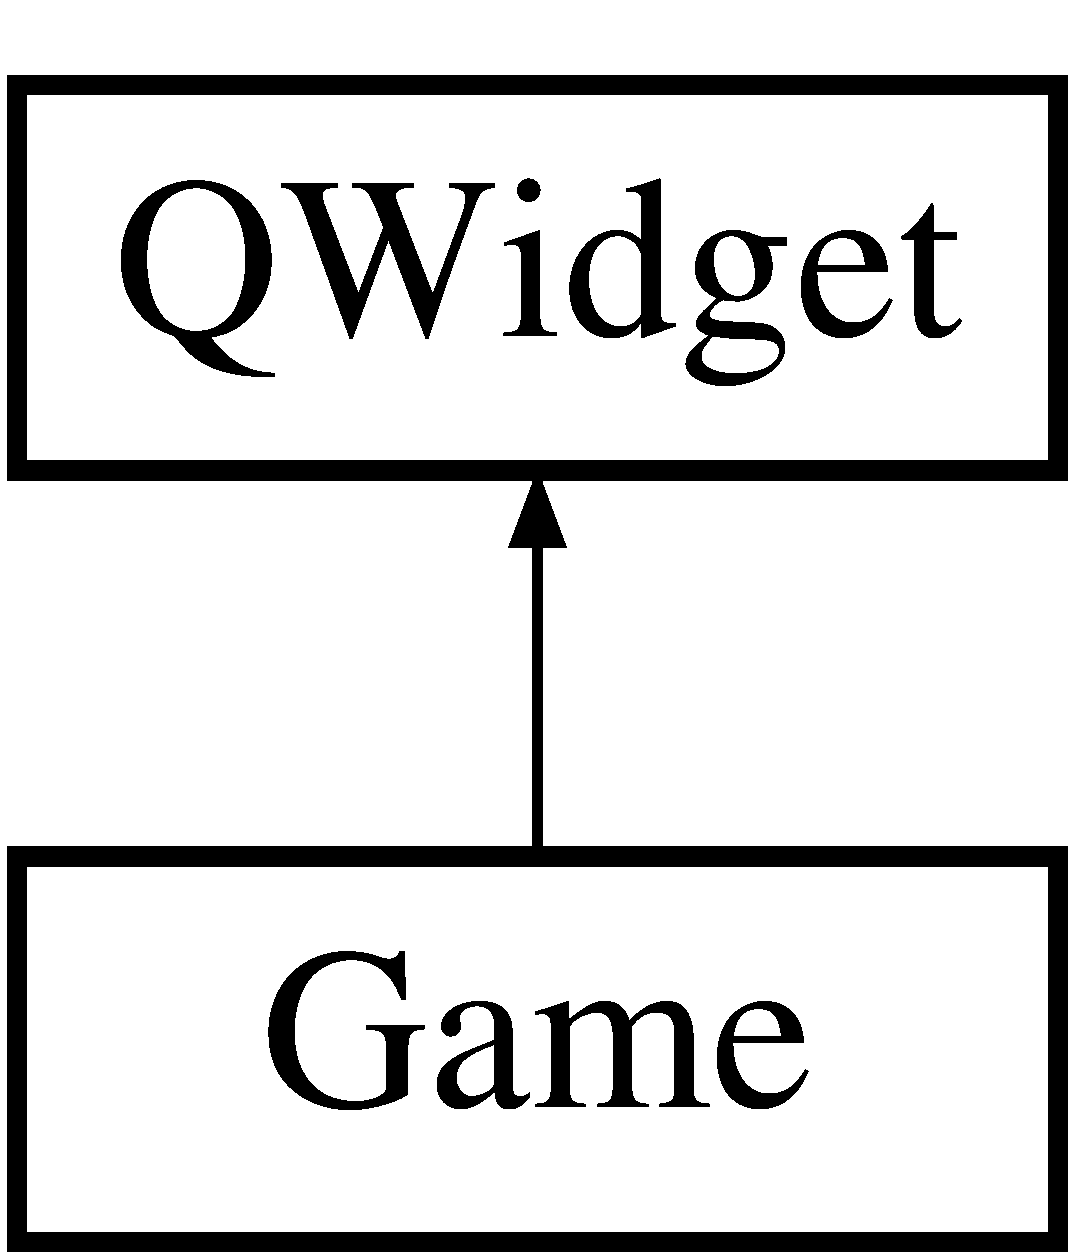
\includegraphics[height=2.000000cm]{class_game}
\end{center}
\end{figure}
\subsection*{Public Slots}
\begin{DoxyCompactItemize}
\item 
void {\bf grow} ()\label{class_game_a95d8530f5a7e1a65250f02b06108d059}

\begin{DoxyCompactList}\small\item\em \doxyref{Game\+::grow}{p.}{class_game_a95d8530f5a7e1a65250f02b06108d059} increment board incriment board after certain time, increment as well all variables in play to keep game working. \end{DoxyCompactList}\end{DoxyCompactItemize}
\subsection*{Public Member Functions}
\begin{DoxyCompactItemize}
\item 
{\bf Game} ()\label{class_game_ad59df6562a58a614fda24622d3715b65}

\begin{DoxyCompactList}\small\item\em \doxyref{Game\+::\+Game}{p.}{class_game_ad59df6562a58a614fda24622d3715b65} game constructor game constructor, load all pictures, start important timers, set rendering engine. \end{DoxyCompactList}\item 
void {\bf delete\+Empty\+Space} ()\label{class_game_ace65c584cceee8977942ace8ad86d080}

\begin{DoxyCompactList}\small\item\em \doxyref{Game\+::delete\+Empty\+Space}{p.}{class_game_ace65c584cceee8977942ace8ad86d080} fix any floating tiles recursive function that fix floating tiles. \end{DoxyCompactList}\item 
void {\bf key\+Press\+Event} (Q\+Key\+Event $\ast$event)
\begin{DoxyCompactList}\small\item\em \doxyref{Game\+::key\+Press\+Event}{p.}{class_game_a08d72c91a6daedc8fa48194253f5e567} key press event, pressing space will start game. \end{DoxyCompactList}\item 
void {\bf mouse\+Press\+Event} (Q\+Mouse\+Event $\ast$event)
\begin{DoxyCompactList}\small\item\em \doxyref{Game\+::mouse\+Press\+Event}{p.}{class_game_a704ba119948eebd1b6dfc547de967796} mouse press event, clicking will change to mouse down game state. \end{DoxyCompactList}\item 
void {\bf mouse\+Move\+Event} (Q\+Mouse\+Event $\ast$event)
\begin{DoxyCompactList}\small\item\em \doxyref{Game\+::mouse\+Move\+Event}{p.}{class_game_ad761e49ff42758930e76b477d08ba068} changing mouse position while pressed will swap tiles swiped across. \end{DoxyCompactList}\item 
void {\bf mouse\+Release\+Event} (Q\+Mouse\+Event $\ast$event)
\begin{DoxyCompactList}\small\item\em \doxyref{Game\+::mouse\+Release\+Event}{p.}{class_game_ae0fc55e9a55fa6c3c44d5a5efa1be987} releasing mouse return to in game state. \end{DoxyCompactList}\end{DoxyCompactItemize}
\subsection*{Protected Member Functions}
\begin{DoxyCompactItemize}
\item 
void {\bf paint\+Event} (Q\+Paint\+Event $\ast$)\label{class_game_ab70cff651797a4eb2b3d1370f3adc7f0}

\begin{DoxyCompactList}\small\item\em \doxyref{Game\+::paint\+Event}{p.}{class_game_ab70cff651797a4eb2b3d1370f3adc7f0} paint event that should be the main painting function but really, we just create the painter here and send it to where the main painting events occur, paint\+Tiles. \end{DoxyCompactList}\end{DoxyCompactItemize}


\subsection{Detailed Description}
The \doxyref{Game}{p.}{class_game} class the main class of game, using mainly Q\+Painter to do all painting. 

\subsection{Member Function Documentation}
\index{Game@{Game}!key\+Press\+Event@{key\+Press\+Event}}
\index{key\+Press\+Event@{key\+Press\+Event}!Game@{Game}}
\subsubsection[{key\+Press\+Event(\+Q\+Key\+Event $\ast$event)}]{\setlength{\rightskip}{0pt plus 5cm}void Game\+::key\+Press\+Event (
\begin{DoxyParamCaption}
\item[{Q\+Key\+Event $\ast$}]{event}
\end{DoxyParamCaption}
)}\label{class_game_a08d72c91a6daedc8fa48194253f5e567}


\doxyref{Game\+::key\+Press\+Event}{p.}{class_game_a08d72c91a6daedc8fa48194253f5e567} key press event, pressing space will start game. 


\begin{DoxyParams}{Parameters}
{\em event} & event handler \\
\hline
\end{DoxyParams}
\index{Game@{Game}!mouse\+Move\+Event@{mouse\+Move\+Event}}
\index{mouse\+Move\+Event@{mouse\+Move\+Event}!Game@{Game}}
\subsubsection[{mouse\+Move\+Event(\+Q\+Mouse\+Event $\ast$event)}]{\setlength{\rightskip}{0pt plus 5cm}void Game\+::mouse\+Move\+Event (
\begin{DoxyParamCaption}
\item[{Q\+Mouse\+Event $\ast$}]{event}
\end{DoxyParamCaption}
)}\label{class_game_ad761e49ff42758930e76b477d08ba068}


\doxyref{Game\+::mouse\+Move\+Event}{p.}{class_game_ad761e49ff42758930e76b477d08ba068} changing mouse position while pressed will swap tiles swiped across. 


\begin{DoxyParams}{Parameters}
{\em event} & event handler \\
\hline
\end{DoxyParams}
\index{Game@{Game}!mouse\+Press\+Event@{mouse\+Press\+Event}}
\index{mouse\+Press\+Event@{mouse\+Press\+Event}!Game@{Game}}
\subsubsection[{mouse\+Press\+Event(\+Q\+Mouse\+Event $\ast$event)}]{\setlength{\rightskip}{0pt plus 5cm}void Game\+::mouse\+Press\+Event (
\begin{DoxyParamCaption}
\item[{Q\+Mouse\+Event $\ast$}]{event}
\end{DoxyParamCaption}
)}\label{class_game_a704ba119948eebd1b6dfc547de967796}


\doxyref{Game\+::mouse\+Press\+Event}{p.}{class_game_a704ba119948eebd1b6dfc547de967796} mouse press event, clicking will change to mouse down game state. 


\begin{DoxyParams}{Parameters}
{\em event} & event handler \\
\hline
\end{DoxyParams}
\index{Game@{Game}!mouse\+Release\+Event@{mouse\+Release\+Event}}
\index{mouse\+Release\+Event@{mouse\+Release\+Event}!Game@{Game}}
\subsubsection[{mouse\+Release\+Event(\+Q\+Mouse\+Event $\ast$event)}]{\setlength{\rightskip}{0pt plus 5cm}void Game\+::mouse\+Release\+Event (
\begin{DoxyParamCaption}
\item[{Q\+Mouse\+Event $\ast$}]{event}
\end{DoxyParamCaption}
)}\label{class_game_ae0fc55e9a55fa6c3c44d5a5efa1be987}


\doxyref{Game\+::mouse\+Release\+Event}{p.}{class_game_ae0fc55e9a55fa6c3c44d5a5efa1be987} releasing mouse return to in game state. 


\begin{DoxyParams}{Parameters}
{\em event} & event handler \\
\hline
\end{DoxyParams}


The documentation for this class was generated from the following files\+:\begin{DoxyCompactItemize}
\item 
game.\+h\item 
game.\+cpp\end{DoxyCompactItemize}

\section{Main\+Window Class Reference}
\label{class_main_window}\index{Main\+Window@{Main\+Window}}
Inheritance diagram for Main\+Window\+:\begin{figure}[H]
\begin{center}
\leavevmode
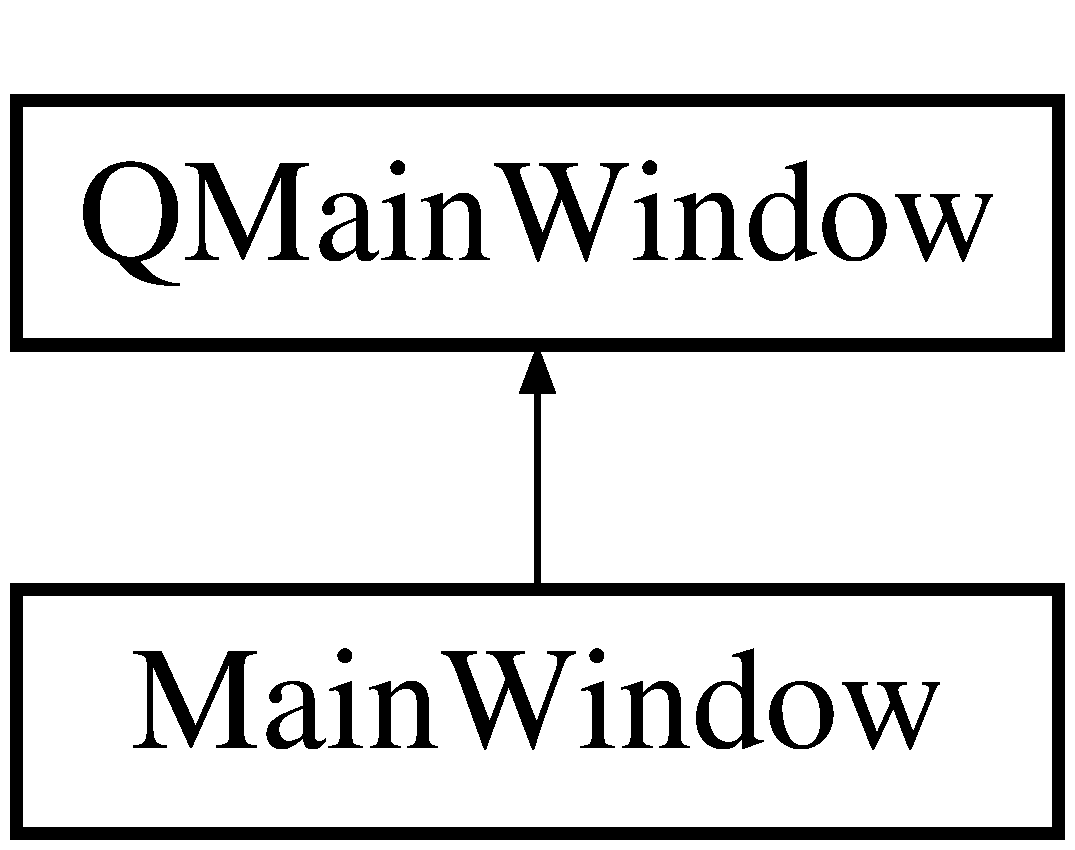
\includegraphics[height=2.000000cm]{class_main_window}
\end{center}
\end{figure}
\subsection*{Public Member Functions}
\begin{DoxyCompactItemize}
\item 
{\bfseries Main\+Window} (Q\+Widget $\ast$parent=0)\label{class_main_window_a8b244be8b7b7db1b08de2a2acb9409db}

\end{DoxyCompactItemize}


The documentation for this class was generated from the following files\+:\begin{DoxyCompactItemize}
\item 
mainwindow.\+h\item 
mainwindow.\+cpp\end{DoxyCompactItemize}

%--- End generated contents ---

% Index
\backmatter
\newpage
\phantomsection
\clearemptydoublepage
\addcontentsline{toc}{chapter}{Index}
\printindex

\end{document}
